\normalsize
\begin{resumoCapitulo}
\textbf{(Resumo opcional no início dos capítulos)} Aqui deve-se escrever um resumo bem pequeno sobre do que se trata o capítulo. O Capítulo XXXX trata dos assuntos x, y, z. Está estruturado da seguinte maneira: Contexto, Motivação, Objetivos, Metodologia e Organização. Se os textos de Objetivos e Metodologia forem pequenos, essas duas seções podem ser agregadas em uma só.
\end{resumoCapitulo}

\section{Exemplo de seção normal} \label{sec:Cap1-Secao1}
\lipsum[1]

\section{Exemplo de seção com o nome muito grande para ocupar mais de uma linha} \label{sec:Cap1-Secao2}
\lipsum[1]

\section{Exemplo de subseções} \label{sec:Cap1-Secao3}

\subsection{Subseção 1.3.1} \label{sec:Cap1-Secao1.3.1}
\lipsum[1]

\subsubsection{SubSubSeção 1.3.1.1} \label{sec:Cap1-Secao1.3.1.1}
\lipsum[1]

\subsection{Subseção 1.3.2} \label{sec:Cap1-Secao1.3.2}
\lipsum[1]

\section{Enumerações} \label{sec:Cap1-Secao4}
\subsection{Itemize}
Certamente o comando mais usado por mim em apresentações, pois trás estrutura de tópicos que é marca caracteristicas de apresentações em slide. O ambiente é muito simples,

\begin{itemize}
	\item Item 1
	\item Item 2
\end{itemize}

\subsection{Enumerate}
Um ambiente muito semelhante ao itemize é o enumerate, a única diferença é a utilização de números ou letras para classificar os itens, ao invés de pontos. Exmplo abaixo mostra a situação:

\begin{enumerate}
   \item item1
   \item item2
 \end{enumerate}

ou:

\begin{enumerate}[a]
	\item Preenchimento com \'Oxido de grafeno
	\item Aquecimento e redu\c{c}\~ao
	\item Desprotegimento do grafeno
	\item Secagem
	\item Remo\c{c}\~ao do Cobre
\end{enumerate}

\subsection{Descrição}
Uma terceira forma de listar é descrevendo os tópicos (pense em um glossário). Fazemos isso com o ambiente description:
\begin{description}
	\item[banana] fruta amarela, a forma lembra a Lua.
	\item[maçã] fruta vermelha e arredondada.
\end{description}

\section{Notas de rodapé} \label{sec:Cap1-rodape}

Criar uma nota de rodapé é simples\footnote{Esse é um exemplo de nota de rodapé.}.

\section{Referências} \label{sec:Cap1-Secao5}
Esse documento usa a biblioteca natbib para a gerenciamento das citações. Para mais exemplos do uso da biblioteca, favor acessar: \url{http://merkel.texture.rocks/Latex/natbib.php}.
\subsection{Citações básicas}
Existem duas formas básicas de citação: citet (para citação textual) e citep (para citação com parêntese). Existe também as versões com * as quais imprimem a lista completa de autores. Todas essas formas podem possuir até 2 argumentos (opcional) para adicionar um texto antes e depois da citação. 
\begin{description}
   \item [\textbackslash citet\{Acree1979\}]= \citet{Acree1979}
   \item [\textbackslash citet{[}capítulo 2{]} \{Acree1979\}]= \citet[capítulo 2]{Acree1979}
   \item [\textbackslash citep\{Acree1979\}]= \citep{Acree1979}
   \item [\textbackslash citep{[}capítulo 2{]}\{Acree1979\}]= \citep[capítulo 2]{Acree1979}
   \item [\textbackslash citep{[}veja{]}{[} {]}\{Acree1979\}]= \citep[veja][]{Acree1979}
   \item [\textbackslash citep{[}veja{]}{[}capítulo 2{]}\{Acree1979\}]= \citep[veja][capítulo 2]{Acree1979}
   \item [\textbackslash citet*\{Acree1979\}]= \citet*{Acree1979}
   \item [\textbackslash citep*\{Acree1979\}]= \citep*{Acree1979}
\end{description}

\subsection{Múltipas citações}
Citando mais de um trabalho de uma vez:
\begin{description}
   \item [\textbackslash citet\{Acree1979,lucredio2009\}]= \citet{Acree1979,lucredio2009}
   \item [\textbackslash citep\{Acree1979,lucredio2009\}]= \citep{Acree1979,lucredio2009}
   \item [\textbackslash citep\{Acree1979,Acree1980\}]= \citep{Acree1979,Acree1980}
   \item [\textbackslash citep\{Acreed1979a,Acreed1979b\}]= \citep{Acreed1979a,Acreed1979b}
\end{description}

\subsection{Citações parciais}
As vezes é necessário citar só parte da referência:

\begin{description}
   \item [\textbackslash citeauthor\{Acree1979\}] = \citeauthor{Acree1979}
   \item [\textbackslash citeauthor*\{Acree1979\}] = \citeauthor*{Acree1979}
   \item [\textbackslash citeyear\{Acree1979\}] = \citeyear{Acree1979}
   \item [\textbackslash citeyearpar\{Acree1979\}]= \citeyearpar{Acree1979}
\end{description}

\section{Figuras} \label{sec:Cap1-Secao6}
Recomenda-se deixar as figuras salvas em uma pasta dentro de cada capítulo, como nesse exemplo.
\begin{figure}[!ht]
	\centering
	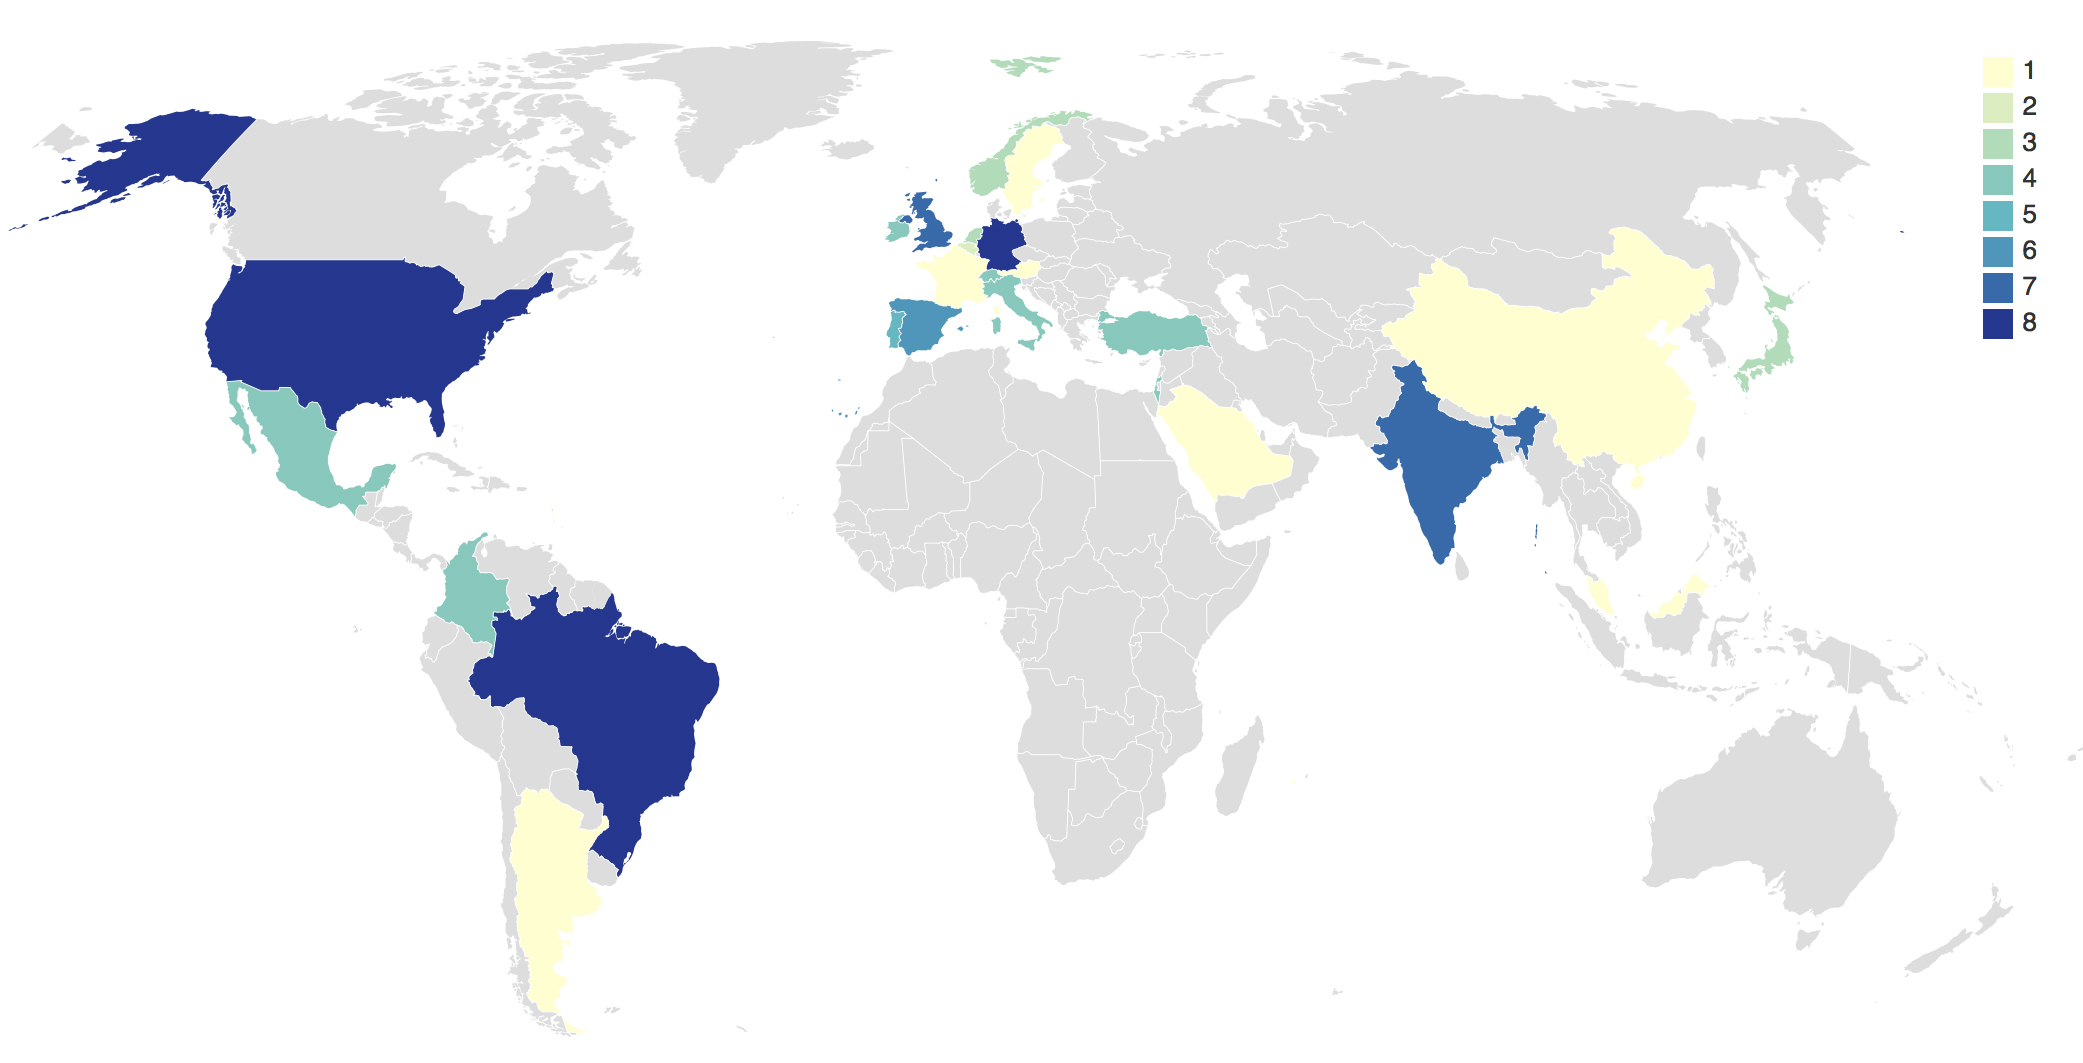
\includegraphics[width=1\textwidth]{Capitulo-1-Exemplo/Figuras/mapa.jpg}
	\caption{Exemplo de uso de Figura}
	\label{Start01}
\end{figure}

\lipsum[1]

\section{Tabelas} \label{sec:Cap1-Secao7}
Recomenda-se deixar as tabelas em arquivos separados e incluí-las como nesse exemplo.
\begin{table}[!ht]

%   float placement
%----------------------
%-h means here: Place the figure in the text where the figure environment is written, if there is enough room left on the page
%-t means top: Place it at the top of a page.
%-b means bottom: Place it at the bottom of a page.
%-p means page: Place it on a page containing only floats, such as figures and tables.
%-! allows to ignore certain parameters of LaTeX for float placement, for example:
%
%	\topfraction: maximal portion of a page (or column resp., here and below), which is allowed to be used by floats at its top, default 0.7
%	\bottomfraction: maximal portion of a page, which is allowed to be used by floats at its bottom, default value 0.3
%	\textfraction: minimal portion of a page, which would be used by body text, default value 0.2
%	\floatpagefraction: minimal portion of a float page, which has to be filled by floats, default value 0.2. This avoids too much white space on float pages.
%	topnumber: maximal number of floats allowed at the top of a page, default 2
%	bottomnumber: maximal number of floats allowed at the bottom of a page, default 1
%	totalnumber: maximal number of floats allowed at whole page, default 3

\setlength{\arrayrulewidth}{2\arrayrulewidth}  % line thickness
\setlength{\tabcolsep}{4pt} % spacing between columns
\centering

\caption{Exemplo de uso de tabelas}
\label{tablePaises}

%\fontencoding{T1}
%\fontfamily{\rmdefault}
\fontseries{m}
\fontshape{n}
%\fontsize{7.75}{8.5}
\selectfont
	\begin{tabular}{lclc}
		\toprule
		Country           & Number & Country         & Number \\ \midrule
		Germany        & 8          & USA          & 8          \\
		Brazil         & 7          & India        & 7          \\
		United Kingdom & 7          & Spain        & 6          \\
		Portugal       & 5          & Colombia     & 4          \\
		Ireland        & 4          & Israel       & 4          \\
		Italy          & 4          & Mexico       & 4          \\
		Switzerland    & 4          & Turkey       & 4          \\
		Japan          & 3          & Netherlands  & 3          \\
		Norway         & 3          & Belgium      & 2          \\
		Argentina      & 1          & Austria      & 1          \\
		China          & 1          & France       & 1          \\
		Malaysia       & 1          & Saudi Arabia & 1          \\
		Sweden         & 1          &              &            \\ \bottomrule
	\end{tabular}
\end{table}



\lipsum[1]

